\documentclass[10pt]{article}
\usepackage{amsmath}
\usepackage{amssymb}
\usepackage{graphicx}
\usepackage{color} % for revision purposes only, may be not present in the final file
% cite package, to clean up citations in the main text. Do not remove.
% \usepackage{cite}
\usepackage{color}
\usepackage{indentfirst} %% LM: in order to indent the first paragraph of each section
\usepackage{url} %% LM: in order to include nice urls
\usepackage{booktabs} %% LM: nice tables...
\usepackage{subfigure} % LM: panels
\usepackage[authoryear,round]{natbib}
\bibliographystyle{apalike}
\usepackage{xr} % automatic cross-referencing
\externaldocument{Text_S2}
% Use doublespacing - comment out for single spacing
%\usepackage{setspace}
%\doublespacing

\topmargin 0.0cm
\oddsidemargin 0.5cm
\evensidemargin 0.5cm
\textwidth 16cm
\textheight 21cm

\usepackage[labelfont=bf,labelsep=period,justification=raggedright]{caption}


\makeatletter
\renewcommand{\@biblabel}[1]{\quad#1.}
\makeatother

\renewcommand{\thesubfigure}{(\Alph{subfigure})}
% Leave date blank
\date{}

\pagestyle{myheadings}
%% ** EDIT HERE **

%% ** EDIT HERE **
%% PLEASE INCLUDE ALL MACROS BELOW

%% END MACROS SECTION

% consistent edits between manuscript and rebuttal letter
%%
%% LaTeX source to reference manuscript changes in revision letters
%%
%% In the manuscript file:
%% 1. Include this file 
%%      %%
%% LaTeX source to reference manuscript changes in revision letters
%%
%% In the manuscript file:
%% 1. Include this file 
%%      %%
%% LaTeX source to reference manuscript changes in revision letters
%%
%% In the manuscript file:
%% 1. Include this file 
%%      \input{make-edits}
%% 2. Define manuscript modifications as
%%      \myedit{UniqueLabel}{Text to appear in manuscript and revision letter}
%%
%% In the revision letter file:
%% 1. Include the automatically updated modifications file
%%      \input{jobname.xtr}
%% 2. Include modified text with
%%      \myeditUniqueLabel
%%
%% Marc A. Suchard
%% 24-Jul-2006
%%

\newwrite\XTR
\AtBeginDocument{\immediate\openout\XTR\jobname.xtr}
\AtEndDocument{\immediate\closeout\XTR}

\newcommand{\myedit}[2]{ % first options is a label, second options is the text
\parbox{0em}{
\shipout\box1{
  \def\mynamea{myedit#1}
  \def\mynameb{\csname \mynamea\endcsname}
\write\XTR{
      \string\newcommand
{\csname myedit#1\endcsname}
}
\write\XTR{
         {``\expandafter\string#2''
         (pg.\string~\thepage)}
}
%\write\XTR{
%    (pg.\string~\thepage)
%}
}
%\hspace*{-1in}
}
%
%\def\thistext{\noexpand#2}
%  \immediate\write\XTR{
%   %     \begin{verbatim}
%        \thistext
%   %     \end{verbatim}
%  }
%\endgroup
%}
%\shipout\vbox{0}
%        \label{\expand\mylabel}
%        \thepage
%  \mylabel
%  \hspace*{-0em}
%  {\bf#2}
#2
}

\newcommand{\myeditblank}[2]{ % first options is a label, second options is the text
\parbox{1em}{
\shipout\box1{
  \def\mynamea{myedit#1}
  \def\mynameb{\csname \mynamea\endcsname}
\write\XTR{
      \string\newcommand
{\csname myedit#1\endcsname}
}
\write\XTR{
         {\expandafter\string#2
         (pg.\string~\thepage)}
}
%\write\XTR{
%    (pg.\string~\thepage)
%}
}
%\hspace*{-1in}
}
%
%\def\thistext{\noexpand#2}
%  \immediate\write\XTR{
%   %     \begin{verbatim}
%        \thistext
%   %     \end{verbatim}
%  }
%\endgroup
%}
%\shipout\vbox{0}
%        \label{\expand\mylabel}
%        \thepage
%  \mylabel
%  \hspace*{-1em}
%  {\bf#2}
}



%\newlength{\strikewidth}
%\newlength{\strikelength}
%\setlength{\strikewidth}{1pt}

%\newcommand{\remove}[1]{
%    \settowidth{\strikelength}{#1}
%    #1\hspace{-\strikelength}
%    \rule[0.5ex]{\strikelength}{\strikewidth}
%}

%\usepackage{ulem}
%\newcommand{\remove}[1]{\sout{#1}}
\newcommand{\remove}[1]{\hspace*{-1em}}

\newcommand{\add}[1]{
%        {\bf #1}
#1%\hspace*{0em}
}


%% 2. Define manuscript modifications as
%%      \myedit{UniqueLabel}{Text to appear in manuscript and revision letter}
%%
%% In the revision letter file:
%% 1. Include the automatically updated modifications file
%%      \input{jobname.xtr}
%% 2. Include modified text with
%%      \myeditUniqueLabel
%%
%% Marc A. Suchard
%% 24-Jul-2006
%%

\newwrite\XTR
\AtBeginDocument{\immediate\openout\XTR\jobname.xtr}
\AtEndDocument{\immediate\closeout\XTR}

\newcommand{\myedit}[2]{ % first options is a label, second options is the text
\parbox{0em}{
\shipout\box1{
  \def\mynamea{myedit#1}
  \def\mynameb{\csname \mynamea\endcsname}
\write\XTR{
      \string\newcommand
{\csname myedit#1\endcsname}
}
\write\XTR{
         {``\expandafter\string#2''
         (pg.\string~\thepage)}
}
%\write\XTR{
%    (pg.\string~\thepage)
%}
}
%\hspace*{-1in}
}
%
%\def\thistext{\noexpand#2}
%  \immediate\write\XTR{
%   %     \begin{verbatim}
%        \thistext
%   %     \end{verbatim}
%  }
%\endgroup
%}
%\shipout\vbox{0}
%        \label{\expand\mylabel}
%        \thepage
%  \mylabel
%  \hspace*{-0em}
%  {\bf#2}
#2
}

\newcommand{\myeditblank}[2]{ % first options is a label, second options is the text
\parbox{1em}{
\shipout\box1{
  \def\mynamea{myedit#1}
  \def\mynameb{\csname \mynamea\endcsname}
\write\XTR{
      \string\newcommand
{\csname myedit#1\endcsname}
}
\write\XTR{
         {\expandafter\string#2
         (pg.\string~\thepage)}
}
%\write\XTR{
%    (pg.\string~\thepage)
%}
}
%\hspace*{-1in}
}
%
%\def\thistext{\noexpand#2}
%  \immediate\write\XTR{
%   %     \begin{verbatim}
%        \thistext
%   %     \end{verbatim}
%  }
%\endgroup
%}
%\shipout\vbox{0}
%        \label{\expand\mylabel}
%        \thepage
%  \mylabel
%  \hspace*{-1em}
%  {\bf#2}
}



%\newlength{\strikewidth}
%\newlength{\strikelength}
%\setlength{\strikewidth}{1pt}

%\newcommand{\remove}[1]{
%    \settowidth{\strikelength}{#1}
%    #1\hspace{-\strikelength}
%    \rule[0.5ex]{\strikelength}{\strikewidth}
%}

%\usepackage{ulem}
%\newcommand{\remove}[1]{\sout{#1}}
\newcommand{\remove}[1]{\hspace*{-1em}}

\newcommand{\add}[1]{
%        {\bf #1}
#1%\hspace*{0em}
}


%% 2. Define manuscript modifications as
%%      \myedit{UniqueLabel}{Text to appear in manuscript and revision letter}
%%
%% In the revision letter file:
%% 1. Include the automatically updated modifications file
%%      \input{jobname.xtr}
%% 2. Include modified text with
%%      \myeditUniqueLabel
%%
%% Marc A. Suchard
%% 24-Jul-2006
%%

\newwrite\XTR
\AtBeginDocument{\immediate\openout\XTR\jobname.xtr}
\AtEndDocument{\immediate\closeout\XTR}

\newcommand{\myedit}[2]{ % first options is a label, second options is the text
\parbox{0em}{
\shipout\box1{
  \def\mynamea{myedit#1}
  \def\mynameb{\csname \mynamea\endcsname}
\write\XTR{
      \string\newcommand
{\csname myedit#1\endcsname}
}
\write\XTR{
         {``\expandafter\string#2''
         (pg.\string~\thepage)}
}
%\write\XTR{
%    (pg.\string~\thepage)
%}
}
%\hspace*{-1in}
}
%
%\def\thistext{\noexpand#2}
%  \immediate\write\XTR{
%   %     \begin{verbatim}
%        \thistext
%   %     \end{verbatim}
%  }
%\endgroup
%}
%\shipout\vbox{0}
%        \label{\expand\mylabel}
%        \thepage
%  \mylabel
%  \hspace*{-0em}
%  {\bf#2}
#2
}

\newcommand{\myeditblank}[2]{ % first options is a label, second options is the text
\parbox{1em}{
\shipout\box1{
  \def\mynamea{myedit#1}
  \def\mynameb{\csname \mynamea\endcsname}
\write\XTR{
      \string\newcommand
{\csname myedit#1\endcsname}
}
\write\XTR{
         {\expandafter\string#2
         (pg.\string~\thepage)}
}
%\write\XTR{
%    (pg.\string~\thepage)
%}
}
%\hspace*{-1in}
}
%
%\def\thistext{\noexpand#2}
%  \immediate\write\XTR{
%   %     \begin{verbatim}
%        \thistext
%   %     \end{verbatim}
%  }
%\endgroup
%}
%\shipout\vbox{0}
%        \label{\expand\mylabel}
%        \thepage
%  \mylabel
%  \hspace*{-1em}
%  {\bf#2}
}



%\newlength{\strikewidth}
%\newlength{\strikelength}
%\setlength{\strikewidth}{1pt}

%\newcommand{\remove}[1]{
%    \settowidth{\strikelength}{#1}
%    #1\hspace{-\strikelength}
%    \rule[0.5ex]{\strikelength}{\strikewidth}
%}

%\usepackage{ulem}
%\newcommand{\remove}[1]{\sout{#1}}
\newcommand{\remove}[1]{\hspace*{-1em}}

\newcommand{\add}[1]{
%        {\bf #1}
#1%\hspace*{0em}
}



\begin{document}

% Title must be 150 characters or less
\begin{flushleft}
{\Large
\textbf{Spatio-temporal Dynamics of Foot-and-Mouth Disease Virus in South America}
}
% Insert Author names, affiliations and corresponding author email.
\\
Luiz Max Carvalho$^{1\ast}$,
Nuno Rodrigues Faria$^{2}$,
Guido K\"onig$^{3}$,
Marc A.~Suchard$^{4,5}$,
Philippe Lemey$^{6}$,
Waldemir de Castro Silveira$^{7}$,
Guy Baele$^{6}$
\\
\bf{1} School of Applied Mathematics, Get\'ulio Vargas Foundation, Rio de Janeiro, Brazil.\\
\bf{2} Department of Zoology, University of Oxford, Oxford, United Kingdom.\\
\bf{3} Institute of Agrobiotechnology and Molecular Biology, INTA-CONICET, Buenos Aires, Argentina.\\
\bf{4} Departments of Biomathematics and Human Genetics, David Geffen School of Medicine at UCLA, University of California, Los Angeles,  United States of America.\\
\bf{5} Department of Biostatistics, UCLA Fielding School of Public Health, University of California, Los Angeles,  United States of America.\\
\bf{6} Department of Microbiology, Immunology and Transplantation, Rega Institute, KU Leuven, Leuven, Belgium.\\
\bf{7} Research and Development Division, Trimatrix Applied Biotechnology Ltd, Rio de Janeiro, Brazil.\\
$\ast$ E-mail: luiz.fagundes@fgv.br
\end{flushleft}
% Please keep the abstract between 250 and 300 words
\section*{Abstract}

\myedit{RefOneComOne}{
Despite  the decrease in incidence of foot-and-mouth disease virus (FMDV) in South America over the last years, the pathogen still circulates in the region and the risk of re-emergence in previously FMDV-free areas is a veterinary public health concern.
In this paper, we employ modern phylodynamic methods to merge epidemiological and genetic data  and reconstruct spatiotemporal patterns and determinants of the dispersal of the two most prevalent FMDV serotypes A and O in South America, while accounting for temporal and spatial sampling bias.
We find that serotypes A and O differ in their temporal pattern of population dynamics, with serotype A displaying more temporal oscillation.
Spatially, we traced the origins of the 2011 Paraguay outbreak to Argentina (posterior probability $0.5$) and Brazil (posterior probability $0.36$). %GB: this seems to be quite a specific statement to be put in the abstract, and it breaks the flow of the abstract in my opinion
Overall, we find that FMDV spread seems to happen mostly through transnational borders, with few long range transmissions, such as a well-supported link between Argentina and Peru for serotype A.
We also found the trade of different livestock (pigs for serotype A and cattle for serotype O) to be associated with viral spread, providing a possible explanation for this pattern of spread.
Our results showcase the usefulness of phylodynamic methods to the study and surveillance of FMDV in South America.
}

Key-words: foot-and-mouth disease virus, South America, animal trade, pathogen phylodynamics, phylogenetics, Bayesian inference, BEAST.

\section*{Introduction}

Foot-and-mouth disease virus (FMDV) is a rapidly evolving picornavirus and the causative agent of foot-and-mouth disease (FMD), the most important disease of domestic and wild cloven-hoofed animals~\citep{Grubman2004}.
The virus can be classified in seven serotypes, three of which (A, O, and C) have circulated in South America.
Serotype A caused large epidemics throughout the Southern cone in recent years~\citep{Perez2001, Malirat2012}, while endemic circulation has been mostly limited to Venezuela~\citep{Malirat2012}.
Historically, serotype O has been the most prevalent serotype on the continent, and was limited to areas in the Andean region, in particular to Ecuador~\citep{Malirat2011}, until recent outbreaks in Colombia~\citep{OIE2017, OIE2018}.
\myedit{RefOneComTwo}{Serotype C on the other hand was last encountered in the continent in $1995$ in Brazil~\citep{Correa2002}.}
Historical reports suggest that FMDV arrived in South America in the late years of the 19th century with European colonization~\citep{Naranjo2013, Tully2008}. 
By the 1970s, FMD was widespread in the region, with several large-scale epidemics being caused by multiple subtypes~\citep{Saraiva2003}.
In South America, FMD control and eradication has traditionally been pursued using a combination of mass vaccination programs~\citep{Saraiva2004b} and control of animal movements from areas in which FMDV infection was suspected.
Over time, passive and active surveillance programs have, with different degrees of success, managed the early detection of FMDV.
In order to achieve complete eradication, however, the strains involved in epidemics - especially those in previously FMDV-free areas - need to be accurately characterised and their temporal and spatial dyamics, studied.

Phylogenetic analyses have proven useful in recovering the transmission pathways from genetic data~\citep{Cottam2008a, Cottam2008b} and in providing insight into the processes that drive re-emergence~\citep{DiNardo2011}.
More recently, molecular epidemiology tools have been used to infer the origin and evolutionary history of emerging strains in South America~\citep{Perez2001, Malirat2007, Malirat2011, Maradei2013}.
However, as pointed out by \citet{DiNardo2011}, a common feature of FMDV molecular epidemiology studies is that joint evaluation of epidemiological, environmental and genetic data has usually been performed outside of a unified quantitative framework.
%GB: how have these studies been performed then and what are the main downsides of not using a unified framework?
The link between phylogenetic analyses and population- and host-specific factors -- such as animal trade and vaccination -- is usually established in a post-hoc rather than a model-based fashion.
In the face of many sources of information, ranging from genetic data to environmental data on host distribution and outbreak counts, it's desirable to have a framework capable of integrating these sources of information coherently~\citep{Lemey2014, Dudas2017}. %GB: we should provide some references - if possible - of studies that don't do this and how they arrived to poor conclusions; probably easier to provide examples that did use proper joint data analysis
%LM: I've patched the text in hopes of adequately (but not brilliantly) addressing this concern

The field of (pathogen) phylodynamics combines population genetics and epidemiology to explicitly  model the interaction between ecological processes such as migration and selection and the shape of the phylogenies~\citep{Grenfell2004, Volz2013, Dudas2017}.
Bayesian phylodynamics offers an attractive statistical framework to combine multiple sources of information while marginalizing over the topology space, thus accommodating phylogenetic uncertainty.
In particular, phylogeographic methods can be employed to understand viral spatial dynamics under explicit spatial diffusion models~\citep{Lemey2009}.
Further, an important research goal is to gain insight into the major determinants of FMDV spread in the continent.
Since human and animal movements constitute a major threat to eradication programs~\citep{Schley2009}, using animal trade data as predictors can be a valuable tool to understand the role of livestock commerce in the spread of FMDV.
For example, \citet{Nelson2011} coupled swine trade data and genetic data to show that swine movements in the United States drove the spread of a novel influenza virus of the H1 subtype while~\cite{Lemey2014} used air travel data to study the driving factors of Influenza H3N2 spread across the globe. 
%GB: should we be more specific here about the actual methodology that was used? after all, neither covariate modelling approaches in BEAST (i.e. for the spatial diffusion and the population size over time) that allow linking these covariates to estimable quantities had been developed yet (Lemey et al. 2014; Gill et al. 2016)?
% LM: Truth is that this Introduction will have to be re-written. This is fossil evidence of the age of the current paper.
% LM: I've patched things up instead of re-writting from scratch. Hope it's OK.

Here, we investigate the phylodynamic patterns of serotypes A and O in South America using all publicly available VP1 (1D) sequences for those serotypes in South America, sampled over a long time-period (1955-2010 for serotype A and 1994-2011 for serotype O) in nearly all south American countries affected by FMD.
We apply Bayesian phylodynamic methods to investigate the evolutionary dynamics of serotypes A and O in South America incorporating  genetic, spatial and epidemiological data such as livestock trade, geographic distances and vaccination coverage.
This flexible Bayesian phylodynamic framework allows for the testing of hypotheses concerning viral dispersal, while naturally accommodating phylogenetic uncertainty~\citep{Lemey2009, Faria2011, Lemey2014, Gill2016}. %GB: update references to include Lemey et al. 2014 and Gill et al. 2016?
% LM Done.
We use BEAST~\citep{Suchard2018} to infer time-structured phylogenies and reconstruct past population dynamics, to which we overlay vaccination and serotype-specific notification data.
To study the factors driving re-emergence, we use data on livestock trade and geographical distances as predictors for viral spatial diffusion and compare competing spatial dynamics models involving each predictor using a generalised linear model approach~\citep{Faria2013,Lemey2014}.
In addtion, we reconstruct the past population dynamics of both serotypes using a sampling-aware method~\citep{Karcher2016,Karcher2020} that takes into account possible temporal sampling bias in the collection of sequences. %GB: be more specific on the 'recently developed methods'
%LM: Added references and a bit of detail.

\section*{Results}

We searched GenBank for FMDV sequences, filtering those that contained the 1D (VP1) gene (over 6,900 sequences) and then keeping those that had location and year of isolation and belonged to South America (see Methods), resulting in final data sets of $184$ ($1955-2013$) sequences for serotype A and $210$ ($1958-2011$) sequences for serotype O.
%%% Trees
The maximum clade credibility (MCC) phylogenetic trees shown in Figure~\ref{fig:trees} point to a considerable amount of geographic movement, as indicated by the interspersing of sequences of different countries.
The tree for serotype A (Figure~\ref{fig:trees}A) shows two major clades that diverge early on, one containing most of the Argentinian sequences, the other clade being more geographically heterogeneous.
For serotype O (Figure~\ref{fig:trees}B), we also notice an early split, with a long-lasting Venezuelan lineage that persisted into the 1970s. 
A major lineage containing all of the Ecuadorian sequences is interspersed with sequences from Colombia.
The time of the most recent common ancestor (tMRCA) for serotype A was estimated at $1919$ ($1903$-$1935$), while the tMRCA for serotype O was estimated at $1946$ ($1924$--$1966$), which covers the date of early sequences from 1958 (excluded from the analyses, see methods).
Relaxed molecular clock analysis showed both serotypes have high substitution rates with the rate estimated at $3.52$ ($2.80$--$4.27$) $\times 10^{-3}$ substitutions/site/year (s/s/y) for serotype A  and at  $5.41$ ($4.00$--$6.92$) $\times 10^{-3}$ s/s/y for serotype O.
Both serotypes showed considerable inter-lineage rate variation with coefficients of variation (posterior mean) of $1$ and $1.6$ for serotypes A and O, respectively.

%%% Skystuff
Reconstructions of past population dynamics for both serotypes under naive and sampling-aware models are presented in Figure~\ref{fig:popdyn}.
The sampling-aware models account for dependence of the sampling process on the underlying effective population size ($N_e(t)$) and other simple time-varying covariates, allowing one to assess the presence of bias.
Results suggest that effective population sizes for serotype A display a pattern of steady increase until circa the 1970s and then steady decline, which then becomes faster closer to the present.
For serotype O, the naive reconstruction, which does not take preferential sampling into account, shows substantial oscillations, not present in the reconstructions using %, warmup = 1000tf
the preferential sampling model.
Reconstructions that do not account for preferential sampling also lead to considerably wider Bayesian credibility intervals.
We used MCC trees obtained from three independent chains per serotype as fixed phylogenies for the population dynamics reconstructions, and results were largely consistent across these replicates. %GB: is such a fixed topology/tree analysis a requirement? I think (but I may have messed up) that I used the model of Karcher et al. in BEAST, accommodating phylogenetic uncertainty? Or is that simply not possible?
%LM: It is indeed possible. The reasons I did not pursue this further are: (i) can only use 'simple' covariates anyway, which is not that interesting and (ii) using the fixed tree approach I could explore simulations to understand robustness, which would take way longer to do with full joint modelling.
In particular, model 3 ($\{\gamma(t), -t, -t^2\}$, see Text S2), which includes both a linear and a quadratic term on the sampling time, yielded the highest (log) marginal likelihood for all three replicates of serotype A and for two of three replicates for serotype O. %GB: this may lead to a discussion, i.e. not all replicates yielded the same results.
For all of the concordant replicates, the smallest log-Bayes factors in support of model 3 were $\approx 9$ for serotype A and $\approx 3$ for serotype O.
This less decisive support in favour of model 3 for serotype O is also manifested in the discrepant replicate, in which model 2, which includes only a linear term on $t$, is favoured with a log Bayes factor of $\approx 1.7$. %GB: this is unclear to me; why is this replicate discrepant? shouldn't that be a sign that we need to increase the computational settings in order to reduce estimator variance?
%LM: In this case, the 'estimator variance' is minuscule, as this relies on marginal likelihoods computed from INLA.These are, however, approximate and that may be the problem here. Or the marginal likelihood displays some dependence on the underlying topology for these models, which would make perfect sense. Maybe material for a future project. For now, I think we're good, but let me know if you feel strongly.

%%% Markov Jumps + BSSVS
Figure~\ref{fig:mj&BFs} shows the network of FMDV spread for both serotypes in South America, reconstructed using Bayesian stochastic search variable selection (BSSVS,~\cite{Lemey2009}) and stochastic mapping~\citep{Minin2008b}. %GB: I believe the term 'stochastic mapping' is in use rather than 'robust counting' for this application of the method.
%LM: Done.
Many connections, for example the Argentina-Brazil, Argentina-Uruguay, Venezuela-Colombia and Brazil-Venezuela links are shared between serotypes, with varying degrees of statistical support.
Overall, connections exist mostly between countries that share borders, and these cross-border connections are mostly concordant across serotypes.
A notable exception is a strong connection between Argentina and Peru for serotype A, which is absent in the network for serotype O.
Peru seems to be a hub for serotype A, with most connections being imports into the country rather than radiating out of it.
When we look at source-sink dynamics by computing the net exchange rate of a country, i.e., the difference between the expected transitions from and to that country, differences between serotypes emerge.
For instance,  Brazil is a sink for serotype A, but acts as a source for serotype O.
The opposite is true for Colombia.
On the other hand, Ecuador is a source and a sink (i.e. a hub) for serotype A, while  Argentina seems to act as both source and a sink for serotype O.
In addition, while the largest positive net exchange rates (imports minus exports) are similar for both serotypes, negative exchange rates differ. %GB: this will require some more explaining, i.e. what are these rates specifically?
%LM: Well, the exchange rates are just what we say they are ``(imports minus exports)''. Why the negative rates differ between serotypes is a mystery to me: (i) could be noise as these matrices are rather small or (ii) it could be that the seeders are always the same, but the receivers (sinks) aren't. This could happen for a myriad of reasons, including trade agreements/bans over time.
Argentina and Colombia are strong sinks for serotype O, but we do not observe a similar pattern for serotype A. 

%%% Epidemic tracing 
We traced the origins of specific epidemics and found that the origin of the 2001 serotype A lies within the root of the tree (Figure~\ref{fig:epidemictracing}A), which indicates that the strains responsible for the 2001 epidemic were likely already present in the country -- which is the most likely state of the root for serotype A.
We traced the MRCA of the 2002 serotype A Ecuadorian epidemic to Brazil with posterior probability $0.52$, while Peru ($0.2$) and Venezuela ($0.17$) were alternative locations of origin (Figure~\ref{fig:epidemictracing}B).
For serotype O, we also traced the origins of the 2002 epidemic in Ecuador, and found overwhelming evidence of a Colombian origin (posterior probability $0.92$, Figure~\ref{fig:epidemictracing}C).
We estimated the most probable location of origin of the serotype O Paraguay 2011 isolate (Figure~\ref{fig:epidemictracing}D) and found that Argentina is the most likely place of origin (posterior probability $0.5$) followed by Brazil ($0.36$, see Discussion).
Tracing the origins of the serotype A 2001 epidemics in Brazil and Uruguay revealed multiple countries of origin (Figure~\ref{sfig:epitrac}A and B), while the Bolivian 2001 strains probably originated in Peru (posterior probability ($0.47$, Figure~\ref{sfig:epitrac}C).
The 2008 strains of serotype A in Colombia and serotype O in Peru can be traced with almost complete certainty to Venezuela and Ecuador, respectively (Figure~\ref{sfig:epitrac}D and F) -- see Lineage 1 in ~\cite{Malirat2012}.

%%% Spatial GLM
To evaluate possible drivers of FDMV spread in South America, we employed the generalised linear model framework of~\cite{Lemey2014}.
The results of this spatial GLM analysis are summarised in Figure~\ref{fig:glm_spatial}, and show that out of $15$ predictors, only the trade of pigs ($1995-2004$) and cattle ($1986-1994$) are significant predictors of spread for serotypes A and O respectively.
However, other predictors that failed to be included with substantial probability, nevertheless yielded posterior 95\% BCIs for the coefficients that exclude zero.
Examples include the product of the number of sequences and pigs trade ($2004-2013$) for serotype A, and the presence of borders, pigs trade ($1995-2004$), product of the number of sequences and number of sequences from the destination location for serotype O (Figure~\ref{fig:glm_spatial}B). %GB: should we mention that the fact that the numbers of sequences not being picked up as significant predictors could be interpreted as signs that worries regarding sampling bias may be unwarranted?

\section*{Discussion}

Dating analyses showed serotype A to be older than serotype O in the continent, a finding consistent with a global analysis of both serotypes~\citep{Tully2008}.
Serotype O also showed remarkably higher substitution rates, but caution should be exercised when interpreting these findings, as the substitution rate is a quantity that incorporates molecular characteristics linked to replication as well as populational processes driving mutation fixation~\citep{Holmes2016}.
Our population dynamics reconstructions suggest that serotype A has experienced a rise and fall trajectory with a sharp increase and subsequent decrease of its effective population size.
Serotype O, in contrast, shows a long period of stability in terms of its population size, followed by a period of decline starting in the mid 1990s. %GB: can we link this to a vaccination program or some other intervention strategy or phenomenon in general?
% LM: Let's wait to see what Andres and Waldemir say.
%LM: I'm none the wiser about this. PL?
Overall, effective population sizes follow the downward trend of FMD case counts shown in Figure~\ref{sfig:case_temporal}, but the limited temporal span of the case data (1990 to 2010) precludes more general conclusions.
\citet{Naranjo2013} provide a longer time series (Figure 3 therein) which shows a spike in cases for serotype A around the mid 1970s and that serotype O cases show a decreasing trend from the 1970s which intensifies around the mid 1990s, which coincides with the start of the decline seen in the left panel of Figure~\ref{fig:popdyn} in the present paper.
Interestingly, the 2001 serotype A epidemic does not seem to lead to noticeable changes in diversity. %GB: what do you mean here? %LM: I mean that such a huge outbreak could lead to a spike in Ne(t), which does not happen.

FMDV spread in South America seems to happen mostly through transnational borders, with long migration routes being rarer.
In keeping with the spatial Bayes factors results (Figure~\ref{fig:mj&BFs}), we found that the presence of borders between countries attained a positive albeit not significant (BF $<3$) coefficient (Figure~\ref{fig:glm_spatial}).
This is specially true for serotype O, for which the 95\% BCI for the coefficient excluded zero (Figure~\ref{fig:glm_spatial}B).
These results are consistent also with the fact that geographic distance yielded a negative coefficient, with the 95\% BCI for serotype O excluding zero.
Taken together, these results indicate that, especially for serotype O, FMDV dispersal takes place over shorter distances, across shared borders and is connected with the trade of live pigs and cattle.
The finding that the Ecuadorian epidemic was most likely seeded from Colombia (Figure~\ref{fig:epidemictracing}C) also suggests an effect of cattle trade, since~\citet{Carvalho2013} show that the origin of the Ecuadorian epidemic was the province of Esmeraldas at the border between the two countries and is where most of the Ecuadorian cattle trade takes place~\citep{Maradei2011}. %GB: source/citation for the final part of this sentence? %LM: Done.
Distance to the border is considered one of the most important factors to FMD spread, at least in the context of the Paraguay/Brazil border~\citep{Amaral2016}.
On the other hand, our finding that Argentina was the most likely origin of the 2011 Paraguayan isolate is in disagreement with~\cite{Maradei2013}, who state that, antigenically, the O/San Pedro/Par/11 isolate is not very similar to Argentinian strains such as O/Corrientes/Arg/06.
We note that out analysis here takes genomic information into account, not just phenotypic traits, which might explain the disagreement.

Figure~\ref{sfig:epitrac}F shows that Ecuador is most certainly the origin of the Peruvian 2008 outbreak, which may be connected with the illegal movement of cattle across the border, as suggested by~\citet{Correa2002}.
Regarding the reservoirs of FMDV in the continent, our results for serotype O partially confirm common knowledge (e.g.\citep{Saraiva2003} and~\citep{Naranjo2013}) that the (possibly illegal) trade of cattle is a driving force of FMDV spread.
On the other hand, our results for serotype A seem to implicate the swine population in the spread of the virus, a mechanism that could be facilitated by swine and caprines only being vaccinated during public health emergencies~\citep{Saraiva2003}.

% \subsection*{Sampling bias}

A crucial goal of the present study was to perform phylodynamic inference while accounting for preferential sampling, both in time and space.
In order to tackle temporal preferential sampling, we have employed a model that explicitly incorporates the sequence sampling dates~\citep{Karcher2020}, while also allowing for the inclusion of covariates to help increase explanatory power.
Our finding that accounting for preferential sampling lead to narrower credibility intervals and better fitting models highlights the dangers of ``naive'' reconstructions based on non-uniform temporal sampling.
In particular, we found that our sampling-aware reconstructions showed fewer oscillations, which could be mistakenly interpreted as genuine changes in population dynamics under a naive model. 
In Text S2, we provide further simulations that investigate the effect of the specific temporal sampling patterns observed for both serotypes when compared to uniform temporal sampling.
%GB: we do not mention nor investigate possible spatial preferential sampling though, but let's stay away from this if possible.
% LM: This is not entirely true. We do investigate spatial preferential sampling by including the appropriate covariates in the spatial genetic GLM. It's just that we report this in the main text, rather than Text S2.

% Spatial: sequences included as predictors in various ways in spatial genetic GLM
To account for spatial preferential sampling, we included the number of sequences isolated in each location as a predictor of spread. 
Since our goal was a conservative analysis, we included the sampling structure in different ways -- difference and product of the number of sequences between countries, numbers of sequences in both origin and destination -- in order to maximise our ability to detect an effect of sampling.
Our results show a mild, not statistically significant effect of sampling as evidenced by the zero-excluding 95\% BCIs obtained for the predictors ``Product \# sequences'' and `` \# sequences destination'' for serotype O.
In addition to~\textit{detecting} spatial preferential sampling, the inclusion of sampling-related predictors allows for~\textit{accommodating} preferential sampling so that other coefficient estimates, made conditionally, are robust to it.

Finally, it is important to point out that differences between serotypes should not be readily attributed to inherent biological differences.
Most inferences reported here depend on complex population-level processes such as the migration of infected hosts, immunological composition of host populations and rearing practices.
As an example, we note that even quantities more strongly linked to molecular processes such as the evolutionary rate depend on population-level processes that obscure or magnify biological differences in mutation rate by influencing rates of fixation.

\subsection*{Limitations of this study}

Sampling-related effects have the potential to lead to incorrect inferences about temporal and spatial patterns in phylodynamic studies~\citep{Hall2016,Dearlove2017}.
As discussed above, we have employed modern statistical methods to quantify and mitigate spatial and temporal preferential sampling in the data analysed in this study.
Despite this, however, we feel it is important to clarify its limitations as they relate to the nature of the sampling process.
We highlight three key limitations, which in our view cannot be completely circumvented by the use of state-of-the-art statistical methods. 
 %  - preferential sampling
First, it is important to understand that while the methods employed in this paper help quantify and account for the effects of preferential sampling, ultimately biased data lack information and hence force us to draw more conservative conclusions.
This is particularly important to consider in light of the fact that early reporting for FMD was not reliable and sampling is likely to be significantly biased downward in the period before 1980s.
% - fragment vs full genome
Secondly, the sequences in the present study are from a particular gene (1D, VP1) rather than the full genomes, for which there are considerably fewer sequences that originate only from a few countries.
This restricts our ability to resolve finer details in the phylogenies and by extension limits the ability of phylodynamic models~\citep{Valdazo2012,Dudas2019}.
% - limited covariate information
A final difficulty we would like to point out is the lack of detailed covariate information, specially negative controls (see~\cite{Dellicour2018} for a description of negative controls in the context of phylogenetic GLMs).
For example, due to the fact that our phylogenies spanned periods of time much longer than the available data, we could not include any temporal predictors of FMDV dynamics. %GB: not sure the term 'temporal predictor' is in use, perhaps explain or phrase differently?
%LM: I happen to think it's unambiguous. Let's see if this confuses people ;-).
In the supplementary material we provide all of the data collected for this study, including data that we could not employ directly, such as vaccination and animal production data.
We hope these data can be of use to other researchers in future studies of more limited temporal and spatial scope.

\section*{Conclusions}

In this paper, we have assembled a large data set of FMDV VP1 gene sequences from South America and employed state-of-the-art statistical methods to analyse the spatiotemporal dynamics of the virus, while accounting for preferential sampling. %GB: not sure I would use the term 'sampling bias' as readers may interpret it from a spatial perspective; perhaps be more specific and talk about preferential sampling more explicitly?
%LM: Agreed. Replaced **all** instances of sampling bias with preferential sampling, including comments =D.
We found that FMDV spread occurs mostly through shared borders and  is connected to livestock trade.
We have traced the origins of several epidemics on the continent, providing valuable information to policy makers.
Ultimately, however, the convenience nature of the sampling process creates biases that cannot be easily accommodated, a problem which is made worse by the sequencing of genes rather than full genomes~\citep{Dudas2019}.
We hope this study showcases the power of phylodynamic methods in aiding epidemiological surveillance of FMD in South America and prompts Public Health agencies to adopt sequencing as an integral part of the surveillance apparatus. 

\section*{Methods}

In this section we detail the computational techniques employed to collect and analyse the data in this paper.
We take a Bayesian approach to parameter inference and statistical testing and all parameter estimates reported in this paper are of the form: posterior mean (95\% credibility interval), unless otherwise stated.

\subsection*{Genetic and epidemiological data}

\textbf{Genetic data.}

We retrieved all FMDV nucleotide sequences available from GenBank~\citep{Benson2013} from the National Center for Biotechnology Information (NCBI, \url{ http://www.ncbi.nlm.nih.gov/}) with more than $600$ bp.
This first step yielded $6, 907$ sequences which were then filtered to exclude all sequences that did not include the 1D (VP1) gene, resulting in $4, 507$ sequences being kept.
We then filtered for sequences from serotypes A and O, yielding $1051$ and $2350$ sequences, respectively.
Next, we excluded sequences that had been extensively passaged in cell culture and selected all sequences from South America (Argentina, Bolivia, Brazil, Colombia, Ecuador, Paraguay, Peru, Uruguay, Venezuela) for which information on country and year of isolation was available.

This resulted in $185$ sequences (from eight countries) for serotype A and $215$ sequences (nine countries) for serotype O, covering time spans of $62$ ($1951$-$2013$) and $53$ (1958-2011) years, respectively (see Tables~\ref{stab:sequences_A} and~\ref{stab:sequences_O} for details).
We aligned each data set using the MAFFT~\citep{Katoh2002} algorithm implemented in the Geneious~\citep{Kearse2012} software package.
After a preliminary phylogenetic analysis (see below), an early serotype A sequence (Venezuela 1951) was excluded because its root-to-tip divergence was incompatible with its sampling date~\citep{Rambaut2016}.
For serotype O, five sequences were excluded under the same criteria (Table~\ref{stab:exclseqs}).
The final data comprised had $184$ ($1955-2013$) and $210$ ($1958-2011$) sequences for serotypes A and O, respectively.

\textbf{Acquisition of trade data.}

Data on animal trade were obtained from the FAO database (\url{http://faostat.fao.org/}).
We retrieved data on the \textit{detailed trade matrix} %GB: this will need more explanation in my opinion
for cattle, pigs and sheep (number of live animals exchanged) covering the period from $1986$ to $2009$, for each of the nine countries.
The detailed trade matrix includes information on export quantity, export value, import quantity and import value for each variable.
We used the information on export and import quantity to compose our predictors.
See Text S2 for more details.
%LM: added more information

\textbf{Vaccination and case data.}

Data on the number of vaccine doses (irrespective of serotype) from 1990 to 2010 were obtained from the PANAFTOSA annual reports (\url{https://www.paho.org/panaftosa/}) and then standardised to doses per (cattle) head in each country.
Serotype-specific outbreak notifications were obtained from FMD Bioportal (\url{http://fmdbioportal.ucdavis.edu:8080/}).

\textbf{Data availability.} All the data used in this paper including BEAST XML files are hosted at~\url{https://github.com/maxbiostat/FMDV_AMERICA}.

In this study we take a Bayesian approach to testing evolutionary hypotheses while accommodating phylogenetic uncertainty.
Details on computational settings and prior choices can be found in Text S2.

\subsection*{Phylogenetic Analysis}

We assume a general time reversible (GTR)~\citep{Tavare1986} model of sequence evolution, along with gamma-distributed rate heterogeneity (4 categories) for all our analyses.
We conducted an initial analysis of the two data sets described, employing PhyML~\citep{Guindon2003} to obtain maximum likelihood phylogenies which we then used in conjunction with Tempest~\citep{Rambaut2016} to produce root-to-tip divergence (RDV) plots and identify discrepant sequences (see~\cite{Rambaut2016} for details).
Having identified considerable rate variation among branches we used the Bayesian Evolutionary Analysis by Sampling Trees (BEAST)~\citep{Suchard2018} software package to infer time-structured phylogenies under relaxed clock models~\citep{Drummond2006}, employing the BEAGLE~\citep{Ayres2012,Ayres2019} library to gain computational efficiency. %GB: update reference to BEAGLE 3
% LM: Done.
%\subsection*{Bayesian model selection}
In order to select an appropriate combination of sequence evolution (Markov), coalescent and relaxed clock models for each data set (see Text S2), we use state-of-the-art marginal likelihood estimators, namely generalised stepping-stone sampling (SS)~\citep{Baele2016} %GB: change publication year to 2016 % LM: Done.
implemented in BEAST~\citep{Suchard2018}.
Following a preliminary Skygrid analysis~\citep{Gill2013}, we selected the constant population size coalescent parametric model -- and its associated working prior -- as the tree prior for these comparisons.

\subsection*{Spatio-temporal Dynamics}

\textbf{Effective population size reconstruction}.

For an initial analysis, we employed the Skygrid coalescent model~\citep{Gill2013,Hill2019} %GB: publication year is wrong? would be nice to cite my protocol paper on the skygrid as well LM: ._.
 to reconstruct the past population dynamics of both serotypes.
Skygrid necessitates the specification of a cutoff value, $K$, commensurate with the age of the root (time to the most recent common ancestor, tMRCA) .
We used $K = 150$ years for serotype A and $K = 100$ for serotype O sets as conservative estimates of the tMRCA of the sampled sequences. 
This demographic prior was used in all subsequent BEAST analysis.

In order to accommodate the effect of preferential (temporal) sampling, we employed the Bayesian Nonparametric Population Reconstruction under Preferential Sampling (BNPR-PS) model of~\cite{Karcher2020} (see also~\cite{Karcher2016}), that accounts for sampling pattern of sequences through an inhomogeneous Poisson process and allows the inclusion of time-varying covariates.
We employed the function \verb|BNPR_PS()| in the~\textbf{phylodyn}~\citep{Karcher2017} R package to fit the preferential-sampling model using three MCC trees derived from previous BEAST analyses. %GB: did a tree already have to be provided for this R analysis? how does this method interact with the BEAST analysis?
%LM: Added a few words answer this.
Both the BNPR and Skygrid models necessitate the estimation of a precision parameter, to which one usually assigns a Gamma distribution with parameters $\alpha = \beta = 0.001$.
In this study however, we employed the penalised complexity (PC) prior of~\cite{Simpson2017}, which has better theoretical properties. %% LM: I have a simulation study and a few analyses to support that claim also, but no need to cite here.
More details on model formulation, testing and comparison are given in Text S2. %GB: is there also a Text S1? LM: No. But there was. So I'll wait until the very end to rechristen Text S2.

\textbf{Reconstructing geographical movements using BSSVS and robust counting}

We employ Bayesian stochastic search variable selection (BSSVS)~\citep{Lemey2009} to compute Bayes factors for migration routes between countries and establish which routes are relevant to the spatial spread of FMDV in South America.
Following the approach of~\citet{Hall2013}, we employ the robust counting technique (Markov jump) of~\cite{Minin2008b} to obtain a probability distribution for the location (country) of origin of each of epidemic.
% Each epidemic is represented by sequences from it, taken as representative (see Text S2 for details). %GB: I don't understand this sentence, can you rephrase? %LM: See below
To represent each epidemic (e.g. Ecuador 2002), we selected a group of representative sequences from that epidemic (country and year) and traced their origins.(see Text S2 for details)

\textbf{Phylogeographic generalised linear models}.

In order to study the influence of different epidemiological predictors on viral diffusion through space, we used information on the trade of live cattle, pigs and sheep divided in three periods ($1986-1995$,~$1996-2004$,~$2005-2013$) for each livestock, resulting in nine predictors. %GB: can this be phrased differently? Do you mean that data for cattle was only available from 1986-1995, pigs for 1996-2004 and sheep for 2005-2013?
%LM: No. For that to be the interpretation I would have to have written 'respectively' in the end. Anyway, added a little bit that should clear things up.
We also included the great circle distance between the (centroids of) countries and the presence/absence of borders between countries as predictors.
Additionally, to assess the influence of sequence (spatial) sampling, we also included the product and absolute differences in sequence (samples) numbers between locations as a predictor of flow (see the appendix in~\cite{Lemey2014} for a discussion).
The numbers of sequences in each location were also included as origin and destination predictors (see~\cite{Dudas2017}), leading to a total of $14$ predictors being considered.
In order to test the relevance of each predictor to spatial spread we used Bayesian stochastic variable selection (BSSVS, \cite{Lemey2009}).
All predictors with the exception of the borders were standard log-transformed. %using $\log(x +1)$ in order to map $0$ to $0$ and standardised to have mean $0$ and standard deviation $1$.
The relevance of each predictor can then be determined using Bayes factors~\citep{KassRaftery1995,Lemey2009,Lemey2014}.
Details are given in Text S2.

\section*{Software versions and computer programs}

%GB: also list BEAGLE?
%LM: Done.
\begin{itemize}
 \item \textbf{PhyML} version 3.0, downloaded from~\url{www.atgc-montpellier.fr/phyml/};
 \item \textbf{Tempest} version 1.5.1, downloaded from~\url{http://tree.bio.ed.ac.uk/software/tempest/}  ;
 \item \textbf{BEAST} version 1.10.4, downloaded from~\url{https://github.com/beast-dev/beast-mcmc/releases/download/v1.10.4/};
 \item \textbf{BEAGLE} version 3.0.0 downloaded from~\url{https://github.com/beagle-dev/beagle-lib/releases};
 \item  \textbf{Jupyter} version 4.4.0, installed from the official Ubuntu repositories;
 \item \textbf{R} version 3.5.0, downloaded from~\url{https://cran.r-project.org/}.
\end{itemize}

All analyses conducted within a GNU/Linux computational environment.
Code to produce many of the plots/analyses is available from~\url{https://github.com/maxbiostat/FMDV_AMERICA}.

\section*{Acknowledgments}
The authors would like to thank Ant\^onio Mendes for clarifications regarding the vaccination data, Matthew Hall, Mandev Gill, Vladmir Minin, Gytis Dudas and Oliver Pybus for insightful discussions and Miguel Carvalho, Felipe Figueiredo and Mauricio Oliveira for operational support.
%We acknowledge the support of the National Evolutionary Synthesis Center (NESCent) through a working group (Software for Bayesian Evolutionary Analysis).

%GB: this will need to be further updated
%LM: this is entirely your big boys' problem. Humble Max here only needs to acknowledge two sources. ;-)
\emph{Funding:} %The research leading to these results has received funding from the European Union Seventh Framework Programme [FP7/2007-2013] under Grant Agreement no. 278433-PREDEMICS and ERC Grant agreement no. 260864.
%This work was also supported by National Institutes of Health grants R01 HG006139 and National Science Foundation grants DMS 1264153.
The research leading to these results has received funding from the European Research Council under the European Union's Horizon 2020 research and innovation programmes (grant agreement no.~725422-ReservoirDOCS).
This work was partially supported by the European Union's Horizon 2020 Research and Innovation Programme under ZIKAlliance Grant Agreement no. 734548 and under VIROGENESIS Grant Agreement no. 634650.
The Artic Network receives funding from the Wellcome Trust through project 206298/Z/17/Z.
PL acknowledges support by the Research Foundation -- Flanders (`Fonds voor Wetenschappelijk Onderzoek -- Vlaanderen', G066215N, G0D5117N and G0B9317N). 
GB acknowledges support from the Interne Fondsen KU Leuven / Internal Funds KU Leuven under grant agreement C14/18/094.


\emph{Conflict of Interest:} none declared

\newpage
\bibliography{FMDV_AMERICA}
% \newpage
% \section*{Figure Legends}
% \newpage
% \section{Figures and Tables}
%%%%%%%%%%%%%%%%%%%%%%%%%%
%%%%%%%%%%%%%%%%%%%%%%%%%%
\begin{figure}[!ht]
\begin{center}
\subfigure[Serotype A]{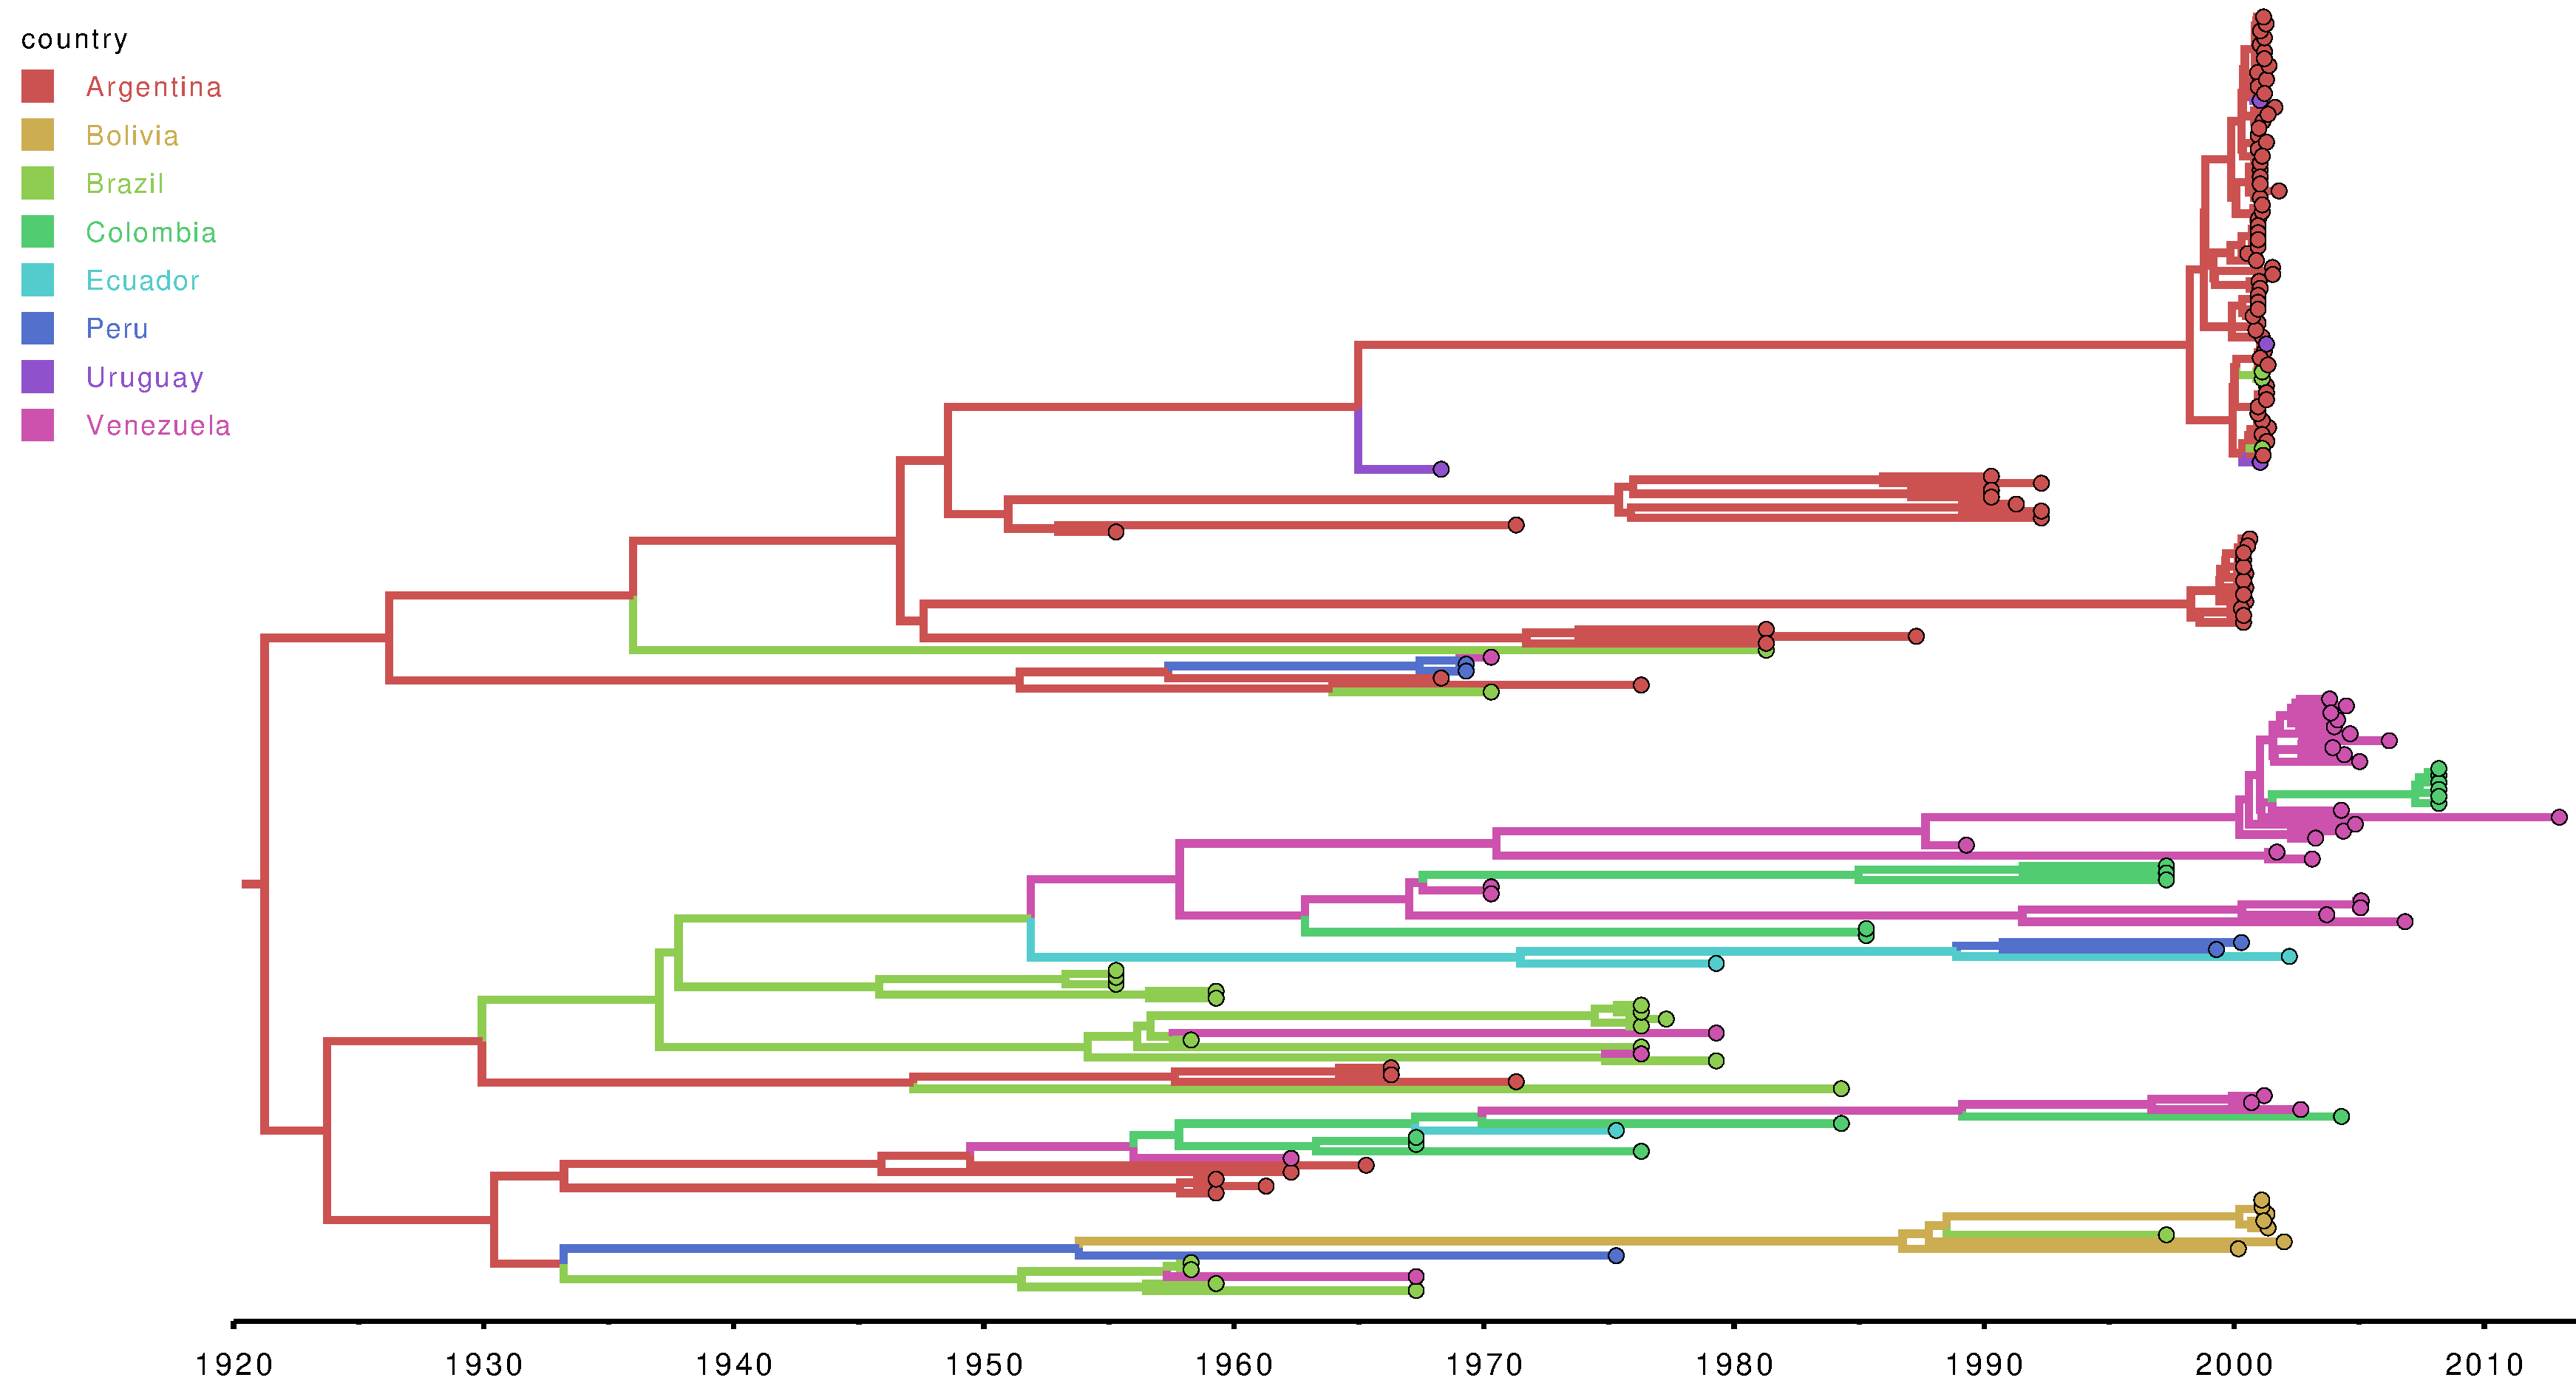
\includegraphics[scale=.25]{FIGURES/PLOTS/tree_A.pdf}}\\
\subfigure[Serotype O]{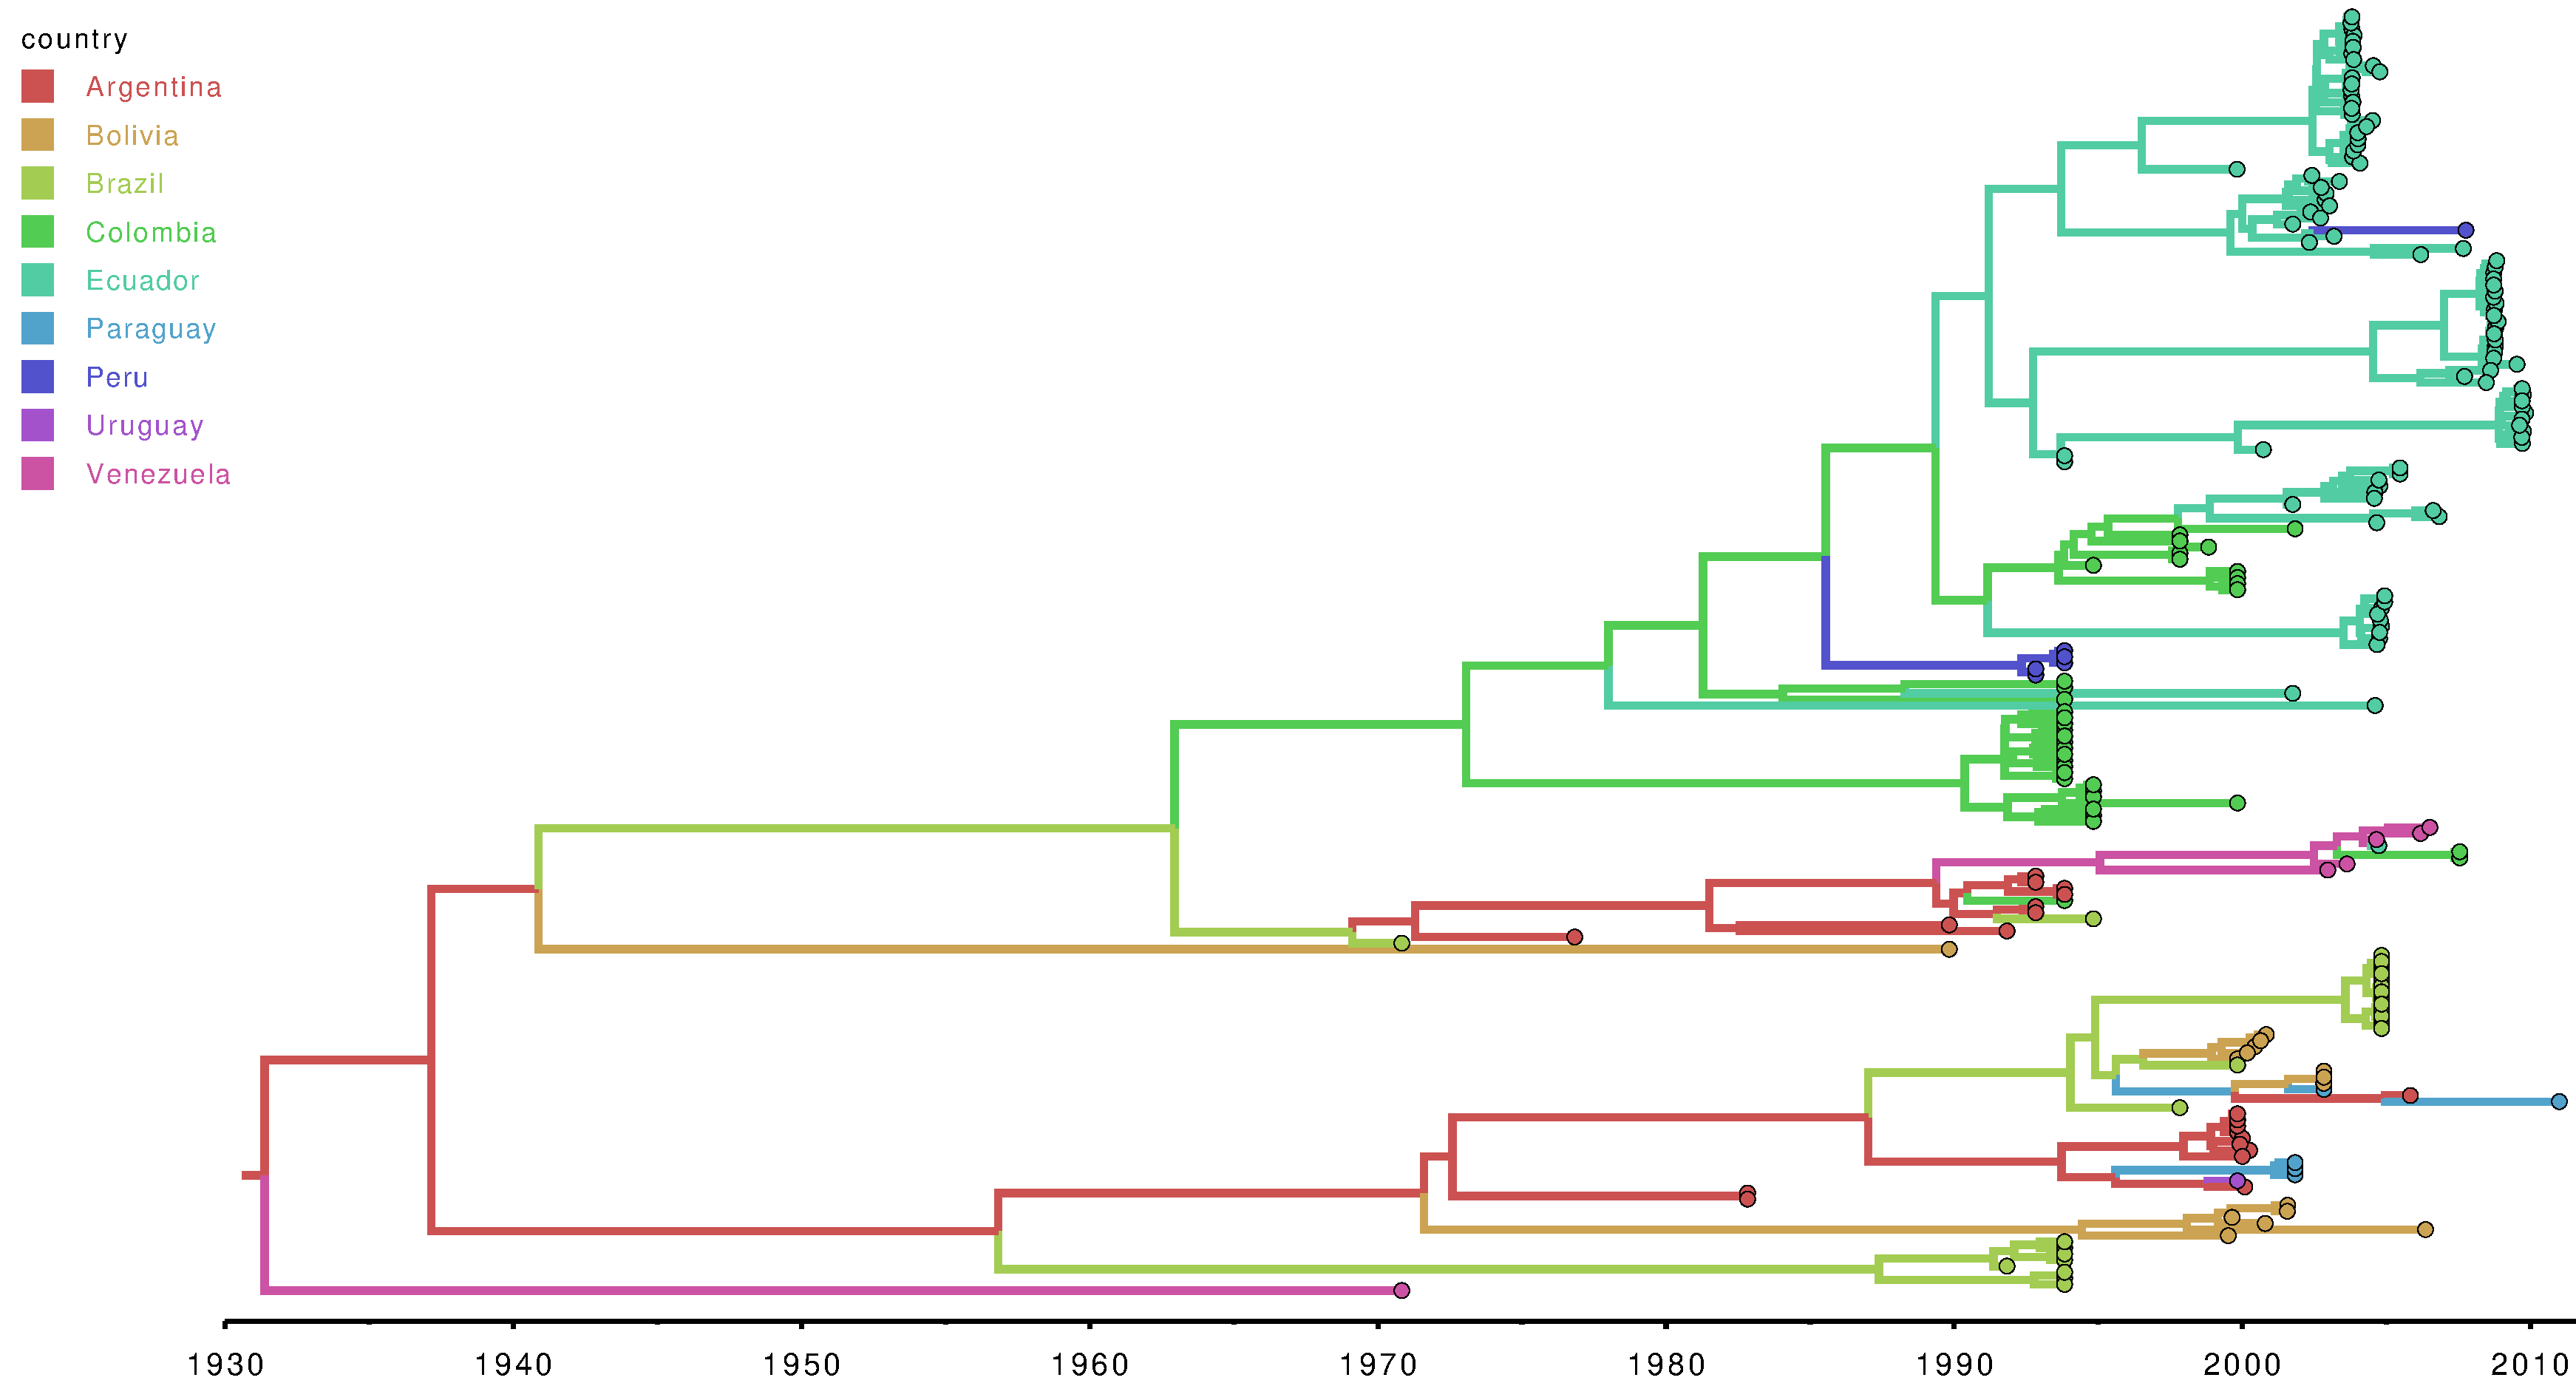
\includegraphics[scale=.25]{FIGURES/PLOTS/tree_O.pdf}} %GB: should we show some measure of uncertainty (for example with respect to the ancestral location states) on the figures?
\end{center}
\caption{\textbf{Maximum clade credibility (MCC) phylogenetic trees reconstructed for FMDV serotypes A and O, with country information mapped}. 
Internal branches are coloured according to the most probable country.
Please notice the slight difference in colour scheme in the legend of both panels. %GB: best to write some text in the caption that discusses the main findings (1 sentence per figure, as you did in the main text)
%LM I'll pass. You're right, but I dislike conclusions/explanations on figure captions. Let's see what the referees say.
}
\label{fig:trees}
\end{figure}
% %%%%%%%%%%%%%%%%%%%%%%%%%%
\begin{figure}[!ht]
\begin{center}
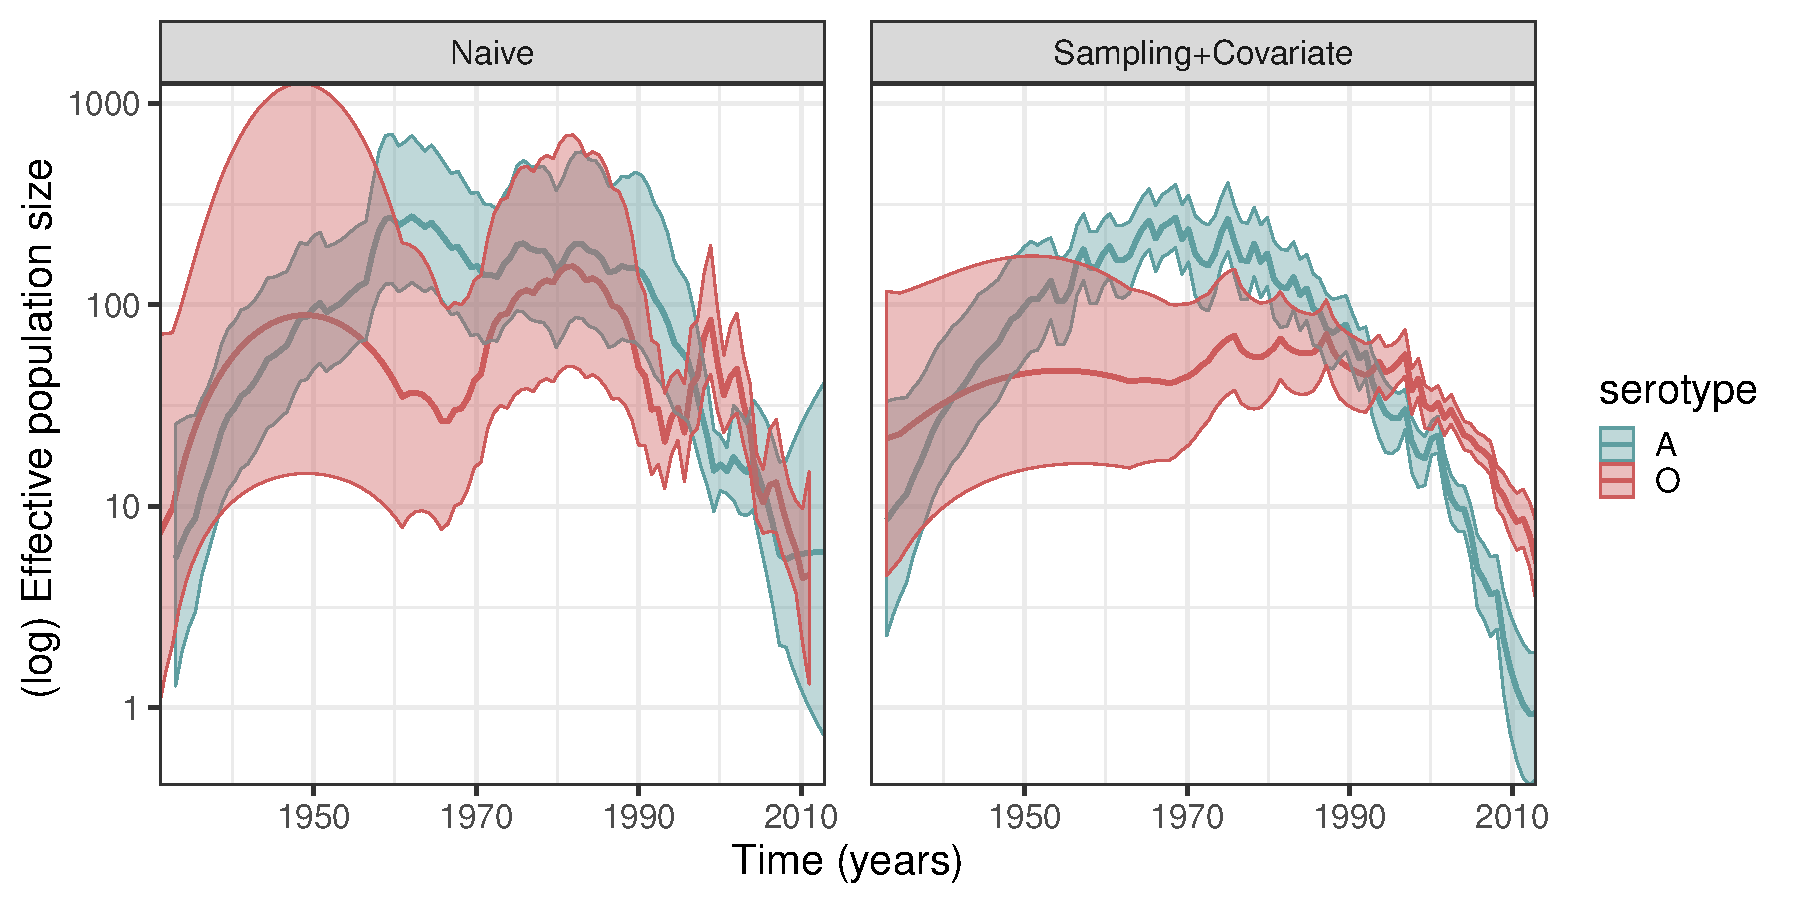
\includegraphics[scale=0.54]{FIGURES/PLOTS/population_size_reconstructions_full.pdf}
\end{center}
\caption{\textbf{Reconstructed population dynamics for serotypes A and O in South America}.
}
In the left panel we show reconstructions that do not take sampling (sequencing) patterns into account, whereas the right panel shows reconstructions using a preferential sampling model~\citep{Karcher2020} that includes a quadratic term on the log-intensity, $\{\gamma(t), -t, -t^2\}$ and which yielded the highest (log) marginal likelihood among the coalescent models tested (see Text S2 for more details).
Colours depict serotypes.

% All estimates were obtained using the \verb|BNPR()| and \verb|BNPR_PS()| functions from the \textbf{phylodyn} package~\citep{Karcher2017}. 
\label{fig:popdyn}
\end{figure}
% %%%%%%%%%%%%%%%%%%%%%%%%%%
\begin{figure}[!ht]
\begin{center}
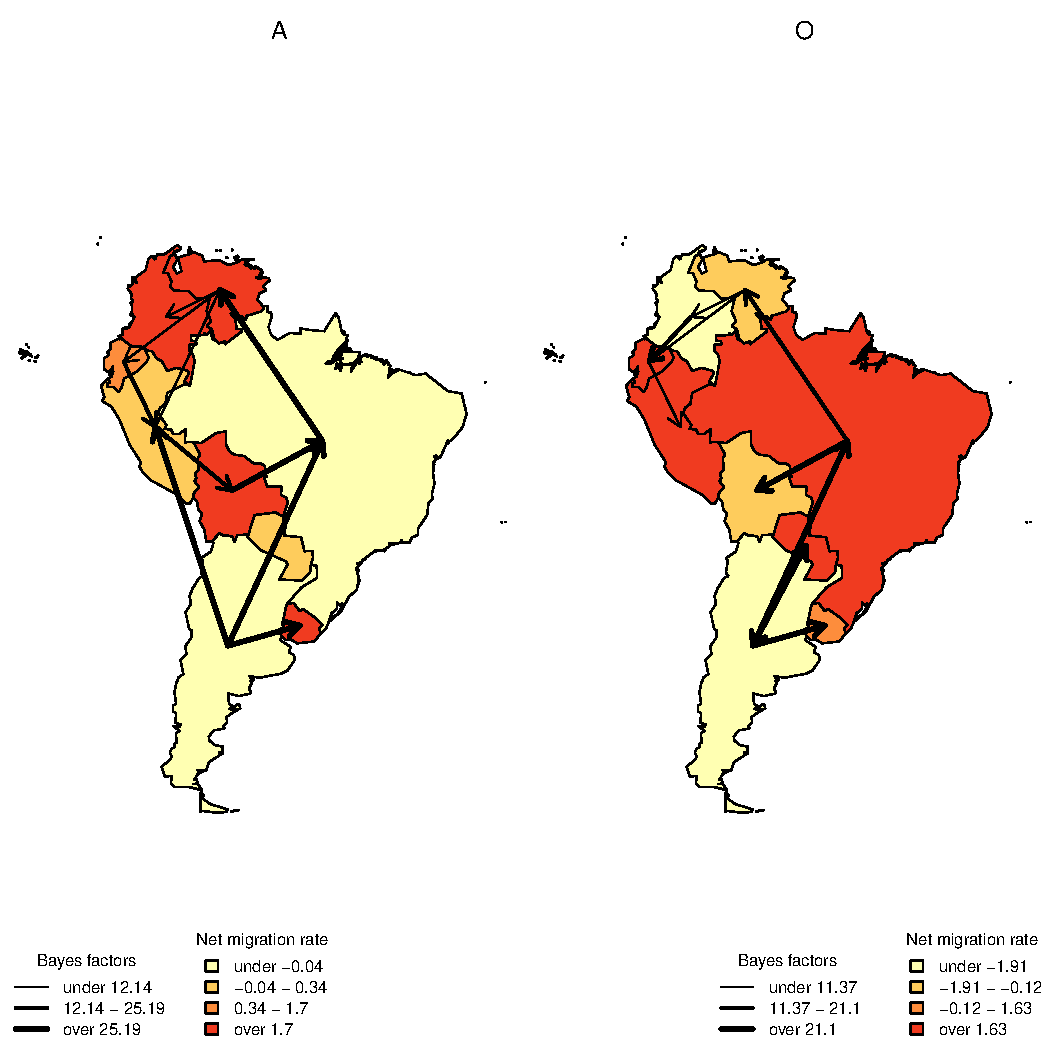
\includegraphics[scale=0.87]{FIGURES/PLOTS/MJandBFs.pdf}
\end{center}
\caption{\textbf{Migration networks for FMDV serotypes A and O in South America}.
We estimate the number of migration events between countries using the robust counting (Markov jumps) technique of~\cite{Minin2008b}.
Additionally, we perform a separate analysis employing Bayesian Stochastic Search Variable Selection (BSSVS) to determine the most significant migration routes.
Bayes factors are depicted by arrows, with line thickness proportional to BF magnitude (we only plot BFs bigger than $3$).
Coroplethic maps show the net migration rates (from - to) for each country but colour scales vary by panel (serotype).
}
\label{fig:mj&BFs}
\end{figure}
% %%%%%%%%%%%%%%%%%%%%%%%%%%
\begin{figure}[!ht]
\begin{center}
\subfigure[][]{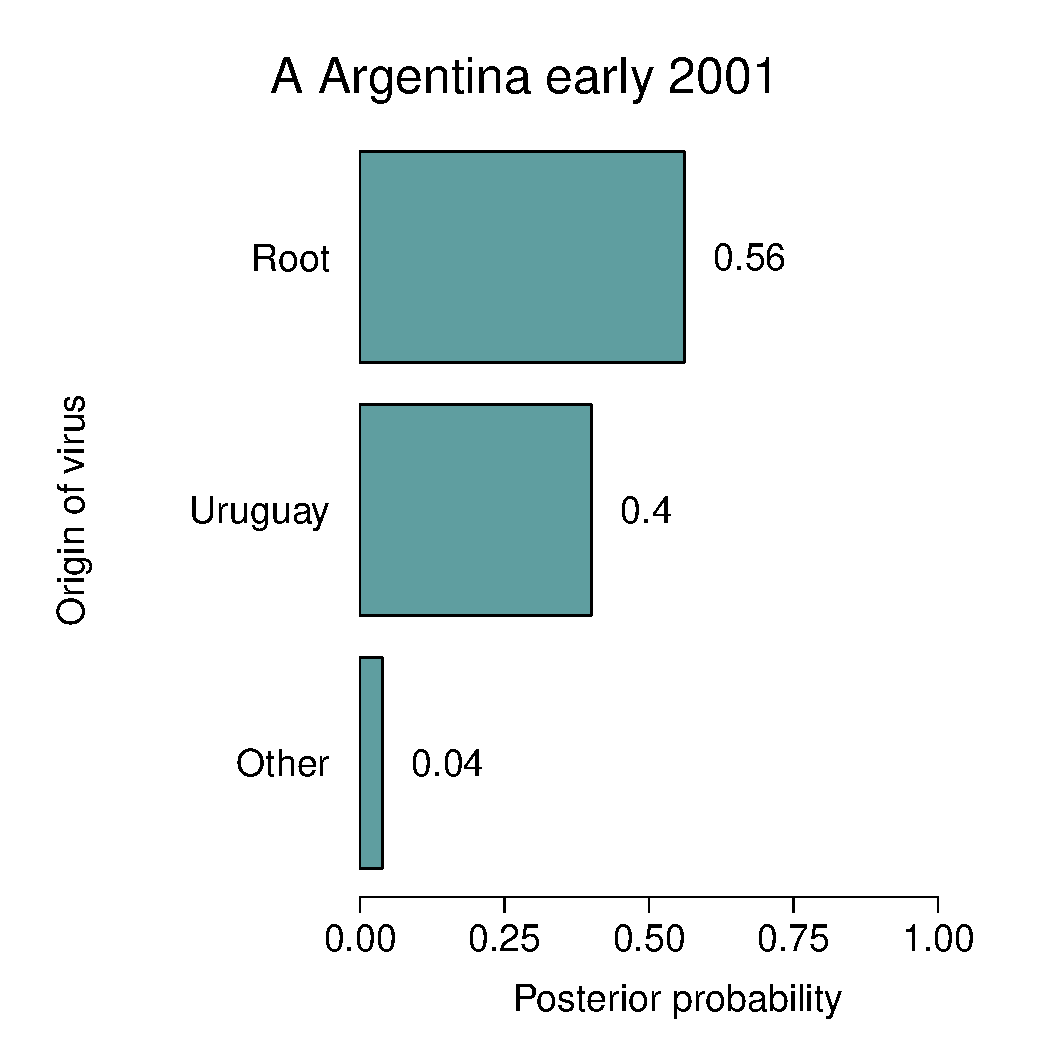
\includegraphics[scale=.40]{FIGURES/PLOTS/Origins_A_Argentina_early_2001.pdf}}
\subfigure[][]{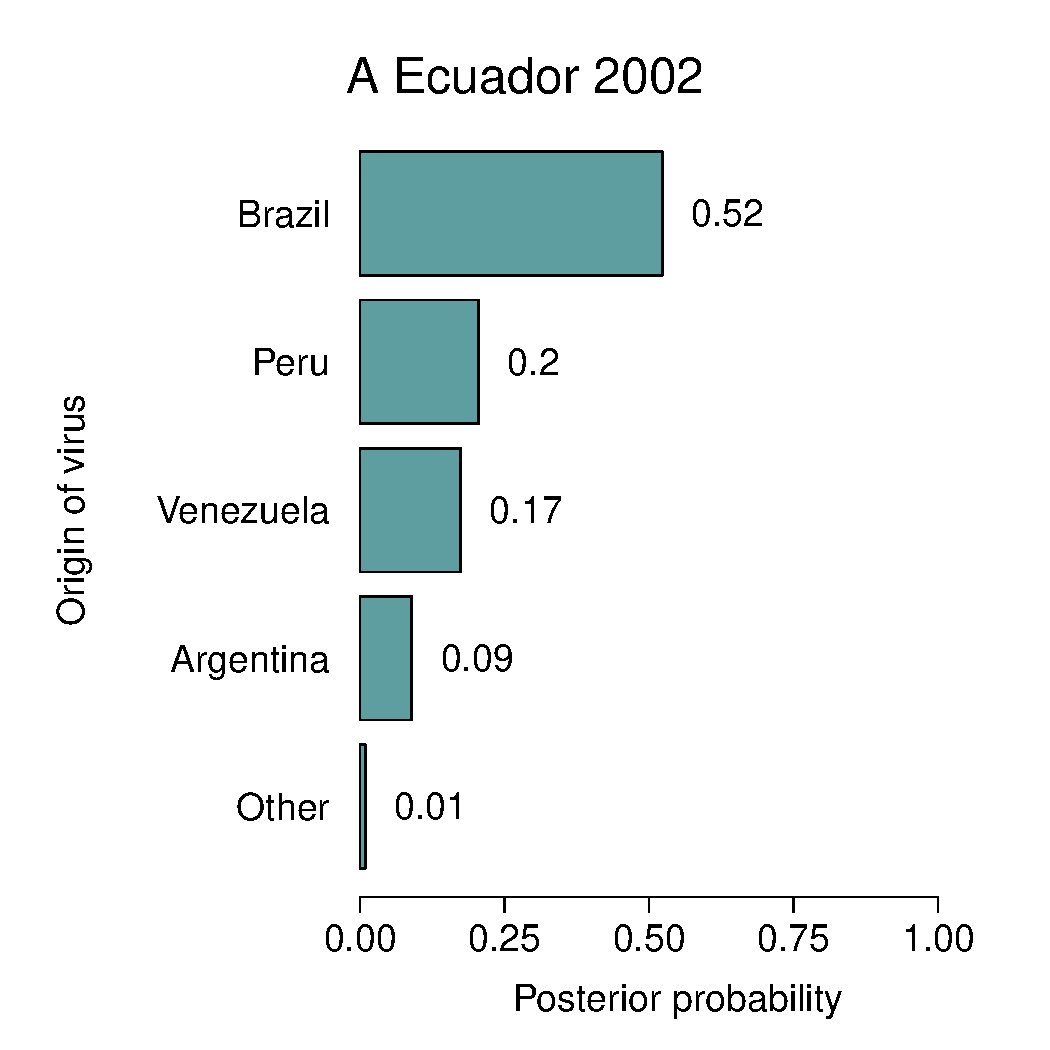
\includegraphics[scale=.40]{FIGURES/PLOTS/Origins_A_Ecuador_2002.pdf}}\\
\subfigure[][]{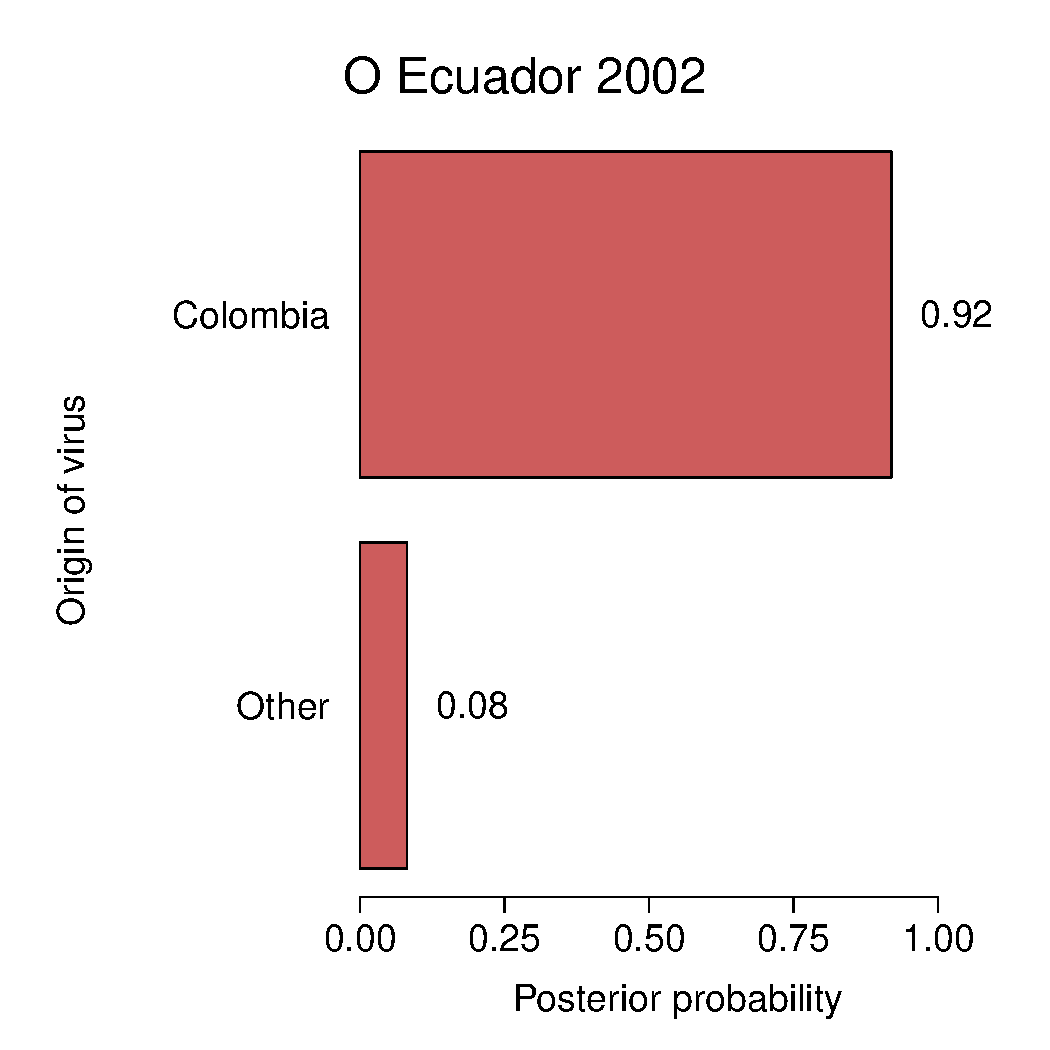
\includegraphics[scale=.40]{FIGURES/PLOTS/Origins_O_Ecuador_2002.pdf}}
\subfigure[][]{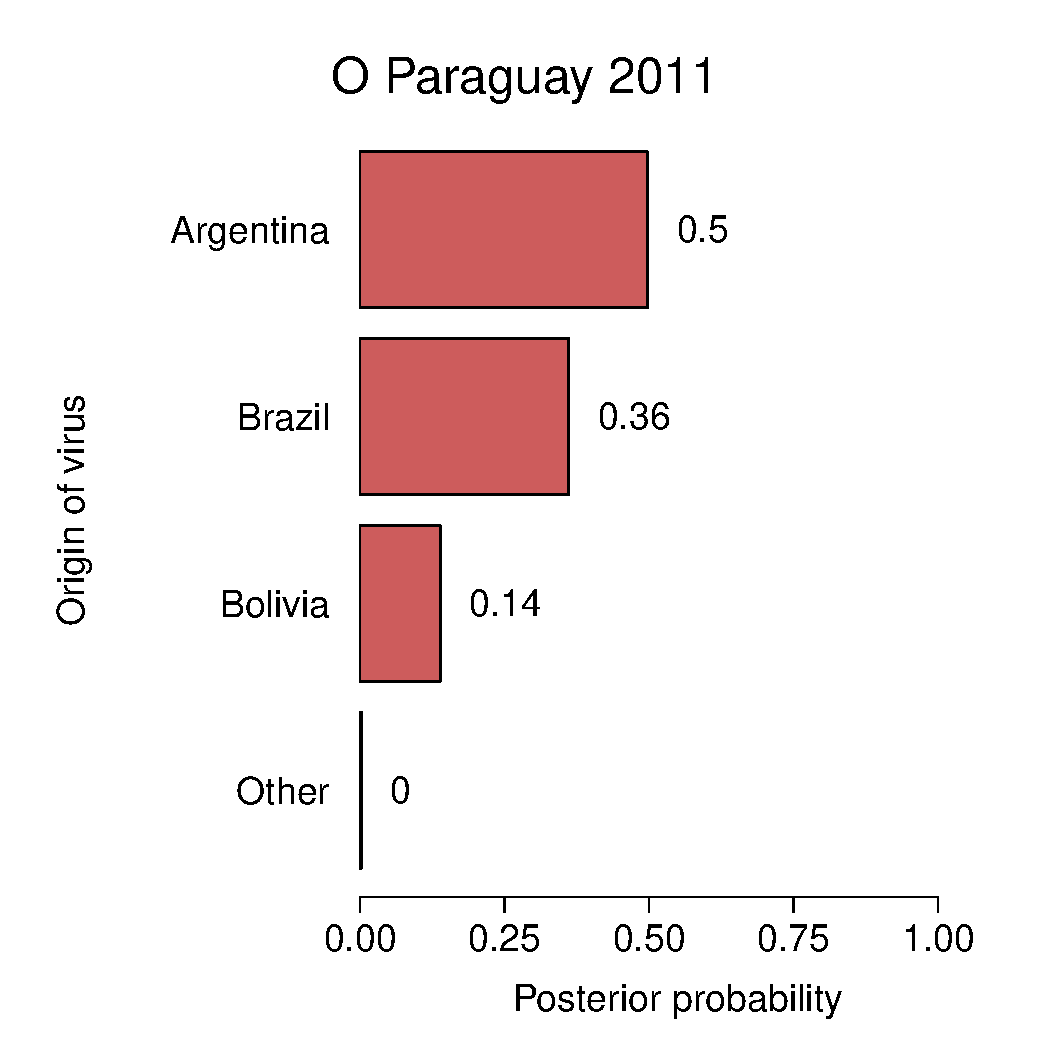
\includegraphics[scale=.40]{FIGURES/PLOTS/Origins_O_Paraguay_2011.pdf}}
\end{center}
\caption{\textbf{Epidemic tracing using robust counting for serotypes A and O in South America}.
We show the most probable sources of serotype A epidemics in Argentina 2001 (A) and Ecuador 2002 (B).
For serotype O the origins of all the Ecuadorian sequences from 2002 (C) are shown along with the origins of the strain in Paraguay 2011 (D).
}
\label{fig:epidemictracing}
\end{figure}
% %%%%%%%%%%%%%%%%%%%%%%%%%%
\begin{figure}[!ht]
\begin{center}
\subfigure[][Serotype A]{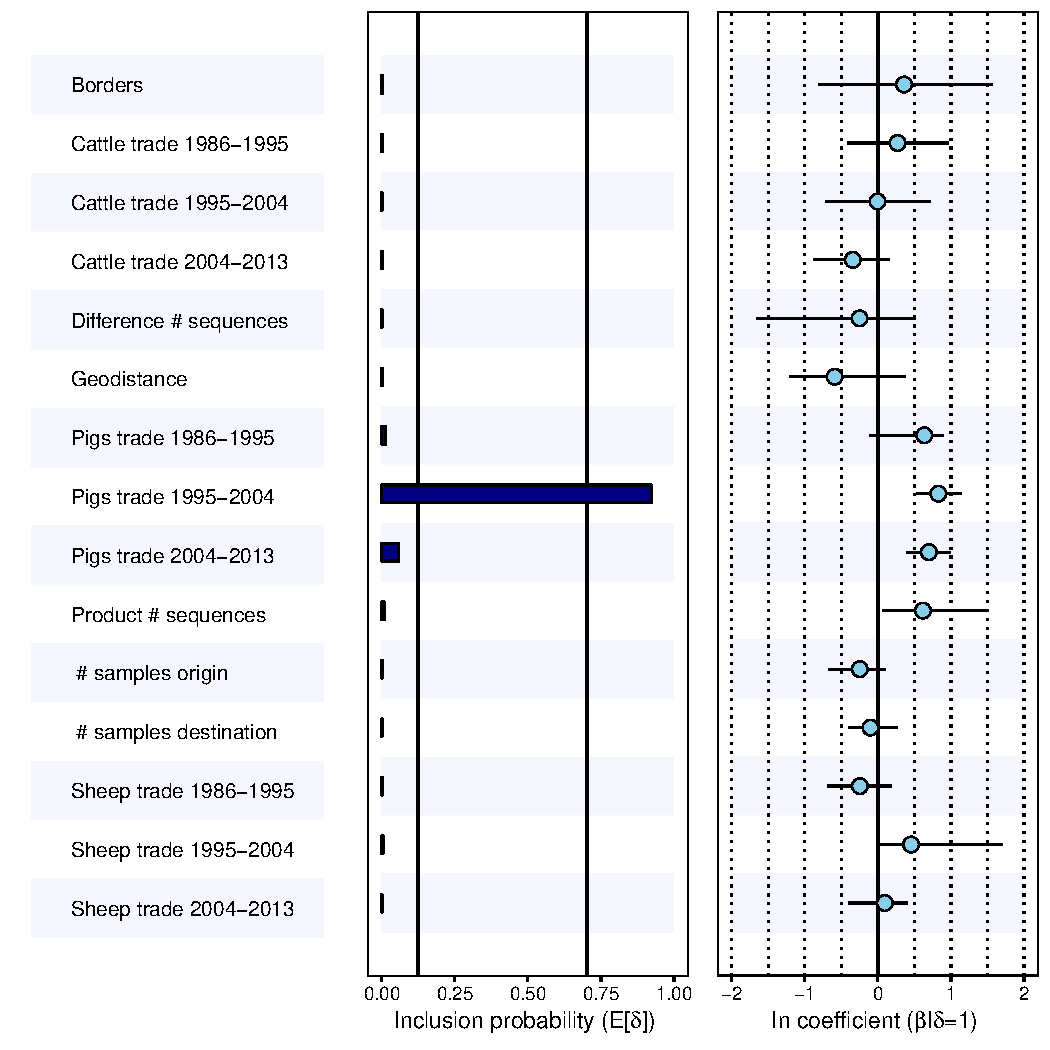
\includegraphics[scale=.50]{FIGURES/PLOTS/glm_A.pdf}}
\subfigure[][Serotype O]{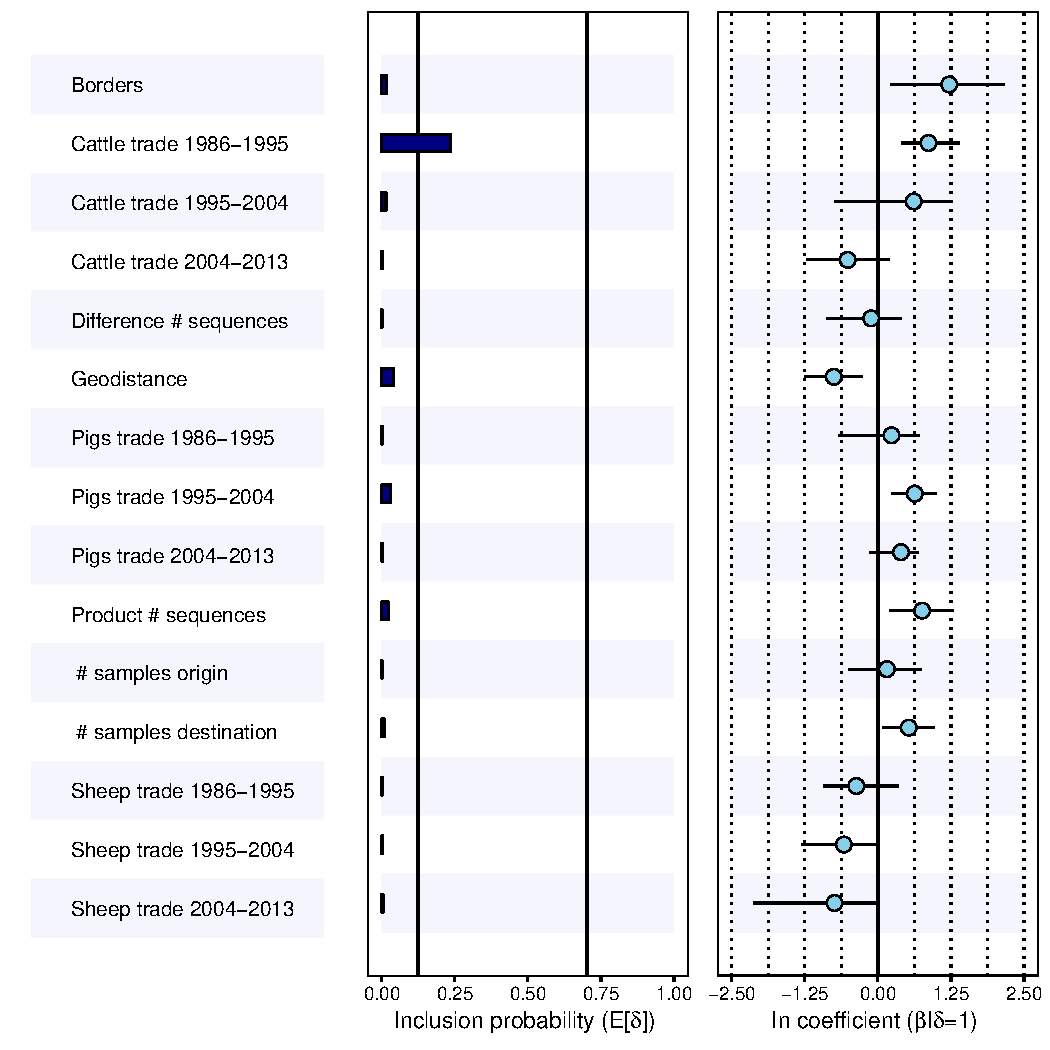
\includegraphics[scale=.50]{FIGURES/PLOTS/glm_O.pdf}}
\end{center}
\caption{\textbf{Phylogeographic generalised linear models for the spatial spread of FMDV in South America}.
We show the inclusion probabilities (posterior mean) and coefficient estimates (mean and 95\% credible intervals) for each of $15$ predictors of spatial spread, for serotype A (panel A) and O (panel B).
Vertical lines on the left subpanel of each plot show the inclusion probabilities corresponding to Bayes factors $3$ and $50$, while the vertical line on the right subpanel marks $\beta | \delta = 0$.
}
\label{fig:glm_spatial}
\end{figure}
\end{document}
